\section{Technical Challenges and Difficulties Encountered}

Developing the core mechanics presented several challenges, particularly regarding entity synchronization and interaction precision.

\subsection{Obstacle Generation Management}
One of the main challenges was designing an \texttt{ObstacleSpawner} capable of generating obstacles at random intervals while maintaining consistent speed for all objects on screen. I had to ensure that obstacle density remained playable despite the randomness, by adjusting the appearance probabilities defined in the project statement (Kebab, Scooter, Student, etc.).

\subsection{Collision Detection with CollisionManager}
Implementing the \texttt{CollisionManager} required special attention. I used Axis-Aligned Bounding Boxes (AABB) for impact detection. The difficulty lay in the polymorphic handling of collisions: the manager must identify the impact, but it is up to each object (\texttt{Obstacle} or \texttt{Player}) to trigger its own behavior (\texttt{onCollision}) according to its nature (health loss, healing, or control inversion).

\begin{figure}[H]
    \centering
    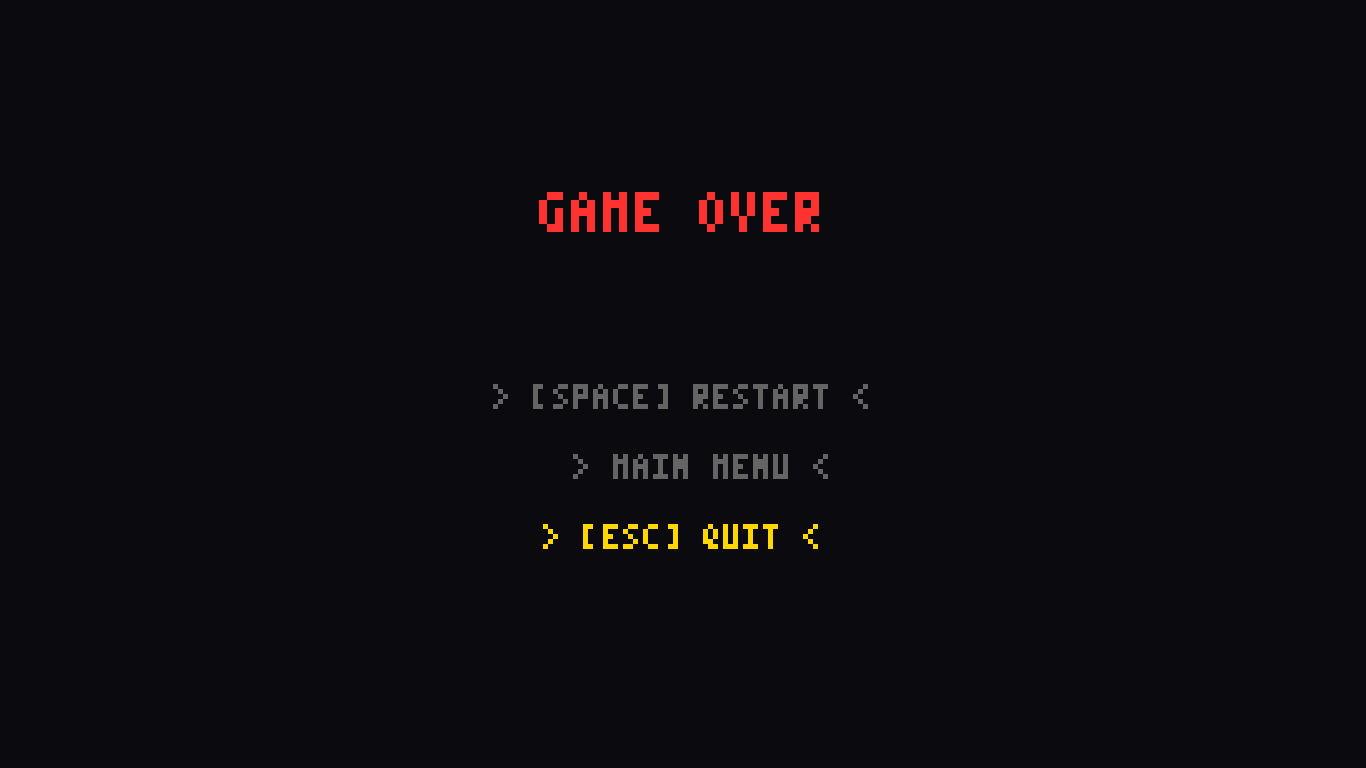
\includegraphics[width=0.6\textwidth]{images/game_over.png}
    \caption{Game over interface showing the final score.}
\end{figure}
